\documentclass{scrreprt}
\usepackage[english]{babel}
\usepackage[T1]{fontenc}
\usepackage{lmodern}
\usepackage{blindtext}
\usepackage[utf8]{inputenc}
\usepackage{siunitx} %For unit handling%
\renewcommand{\familydefault}{\sfdefault}
\newcommand{\unit}[1]{\ensuremath{\, \mathrm{#1}}}
\usepackage{amssymb, amsmath, cancel, ulem, graphicx, float, tabularx}
\usepackage{amsmath}

\setcounter{secnumdepth}{5}
\setcounter{tocdepth}{5}

\author{Urs Gerber\\09-921-156 \and Gian-Luca Mateo\\11-113-545}
\date{28th of February 2013}

\title{Galton Box $\cdot$ Dice $\cdot$ Fall Time}
\subtitle{Practical course report}

\begin{document}
\maketitle

\tableofcontents

\newpage

%-------------------------------Galton Box-----------------------------------%
\chapter{Statistical Toolbox}
For all experiments we used the following universally applicable formulae to calculate the statistical properties of our measurements
\begin{center}
    \begin{tabular}{lcl}
    $x_i$ & : & Samples\\
	$\overline{x}$ & : & Mean of all samples\\
	$N$ & : & Number of samples
\end{tabular}
\end{center}

\paragraph*{Mean}
\begin{equation}
\overline{x}:=\frac{\sum_{i=1}^N{x_i}}{N}
\end{equation}

\paragraph*{Standard deviation}
\begin{equation}
s_x:=\sqrt{\frac{1}{N-1}\sum_{i=1}^N{(x_i-\overline{x})^2}}
\end{equation}

\paragraph*{Standard error of the mean}
\begin{equation}
s_{\overline{x}}:= \frac{1}{\sqrt{N}} s_x
\end{equation}

\chapter[Galton Box]{Galton Box (60 min)}
\section{Introduction}
\subsection{Experiment Goal}
The ball distribution in a Galton Box is a prime example of a binomial distribution. The Goal of this experiment is to show any anomalies and/or build defects of the boxes using statistical means.
\subsection{Theory}
In order for a ball to reach a certain slot, it needs to fall a certain number of times to a certain side of a pin. The number of ways a ball can take to reach a certain slot is described by the formula:
\[\binom{n}{k}=\frac{n!}{(n-k)!k!}\]
were $n$ is the number of slots and $k$ the number of a slot.
This is explained by the fact that in order to reach a certain slot, only the amount of falls in a certain direction is relevant, not the order.

\subsubsection{Preliminary Exercises}
The first thing to show is why we expect the distribution of the balls in the slots to be symmetric. This is easily shown by calculating the amount of possible ways a ball can take to a certain slot($\binom{n}{k}$, where $n$ is the number of slots and $k$ the position of the slot) and showing that it is equal to its opposite in relation to the center ($\binom{n}{n-k}$).
\paragraph*{Task 1}
\begin{equation}
\binom{n}{k} = \frac{n!}{k!(n-k)!} \stackrel{k\rightarrow n-k}{=} \frac{n!}{(n-k)!(\cancel{n}-\cancel{n}+k)!} = \binom{n}{n-k}
\end{equation}
The next few exercises convey some basic ways of handling binomial distributions

\paragraph*{Task 2}
\begin{equation}
2^n = (1+1)^n = \sum\limits_{k=0}^{n}\binom{n}{k} \cdot 1^k \cdot 1^{n-k} = \sum\limits_{k=0}^{n}\binom{n}{k}
\end{equation}

\paragraph*{Task 3.1}
\begin{align}
k \cdot \binom{n}{k} &= \frac{k \cdot n!}{k!(n-k)!} = \frac{n!}{(k-1)!(n-k)!} \notag \\ 
&= \frac{n \cdot (n-1)!}{(k-1)!((n-1)-(k-1))!} = n \cdot \binom{n-1}{k-1}
\end{align}

\paragraph*{Task 3.2}
\begin{align}
k^2 \cdot \binom{n}{k} &= k \cdot n \cdot \binom{n-1}{k-1} \notag \\
&= (k-1+1) \cdot n \cdot \binom{n-1}{k-1} \notag\\
&= (k-1) \cdot n \cdot \binom{n-1}{k-1} + n \cdot \binom{n-1}{k-1} \notag\\
&= n \cdot (n-1) \cdot \binom{n-2}{k-2} + n \cdot \binom{n-1}{k-1}
\end{align}

\paragraph*{Task 4}
\begin{align}
\sum\limits_{x=0}^{n} P_n(x) &= \sum\limits_{x=0}^{n} \binom{n}{x} p^x \cdot q^{n-x} \notag\\
&=(p+q)^n = 1^n = 1
\end{align}

\paragraph*{Task 5}
\begin{equation}
p = (\frac{2}{3})^{3} \cdot \frac{1}{3} \binom{4}{3} = 4 \cdot \frac{8}{27} \cdot \frac{1}{3} = \frac{32}{81}
\end{equation}

\paragraph*{Task 6}
\begin{equation}
\binom{8}{5} = 56
\end{equation}

\subsubsection{Expectations}
\paragraph*{Task 7}

\begin{equation}
F(x) = N \cdot P(x) = N \cdot \binom{14}{x} \cdot 0.5^x \cdot 0.5^{14-x} = N \cdot \binom{14}{x}\cdot 0.5^{14}
\end{equation}

We expect the following occupations per slot for $N=50$ and $N=1000$

% Table generated by Excel2LaTeX from sheet 'Sheet1'
\begin{table}[H]
  \centering
    \begin{tabular}{|l|rr|}
    \hline
    \multicolumn{1}{|r}{\textbf{Slot}} & $N=50$ & $N=1000$ \\
    \hline
    \multicolumn{1}{|c|}{\textbf{0}} & 0.0031 & 0.0610 \\
    \multicolumn{1}{|c|}{\textbf{1}} & 0.0427 & 0.8545 \\
    \multicolumn{1}{|c|}{\textbf{2}} & 0.2777 & 5.5542 \\
    \multicolumn{1}{|c|}{\textbf{3}} & 1.1108 & 22.2168 \\
    \multicolumn{1}{|c|}{\textbf{4}} & 3.0548 & 61.0962 \\
    \multicolumn{1}{|c|}{\textbf{5}} & 6.1096 & 122.1924 \\
    \multicolumn{1}{|c|}{\textbf{6}} & 9.1644 & 183.2886 \\
    \multicolumn{1}{|c|}{\textbf{7}} & 10.4736 & 209.4727 \\
    \multicolumn{1}{|c|}{\textbf{8}} & 9.1644 & 183.2886 \\
    \multicolumn{1}{|c|}{\textbf{9}} & 6.1096 & 122.1924 \\
    \multicolumn{1}{|c|}{\textbf{10}} & 3.0548 & 61.0962 \\
    \multicolumn{1}{|c|}{\textbf{11}} & 1.1108 & 22.2168 \\
    \multicolumn{1}{|c|}{\textbf{12}} & 0.2777 & 5.5542 \\
    \multicolumn{1}{|c|}{\textbf{13}} & 0.0427 & 0.8545 \\
    \multicolumn{1}{|c|}{\textbf{14}} & 0.0031 & 0.0610 \\
    \hline
    \end{tabular}%
\end{table}%

Using 
\begin{equation}
\mu = \sum_{x=0}^n{x F(x)}/N = p n = 7
\end{equation}

and 
\begin{equation}
\sigma^2=\sum_{x=0}^n{F(x)(x-\mu)^2}/N = n p q
\end{equation}

as well as 

\begin{equation}
\sigma_{\mu} = \frac{\sigma}{\sqrt{N}}
\end{equation}

we can calculate 

\[\mu = 7, \quad \forall N \in \mathbb{N}\]
and
\paragraph*{Task 9} 

\begin{align*}
 \sigma_{\mu} &= 1.871 \quad N =1\\
 \sigma_{\mu} &= 0.265 \quad N =50\\ 
 \sigma_{\mu} &= 0.059 \quad N =1000  
\end{align*}

\newpage

\section[The Experiment]{Experiment Assembly and Execution}
\begin{figure}[H]
    \center   
        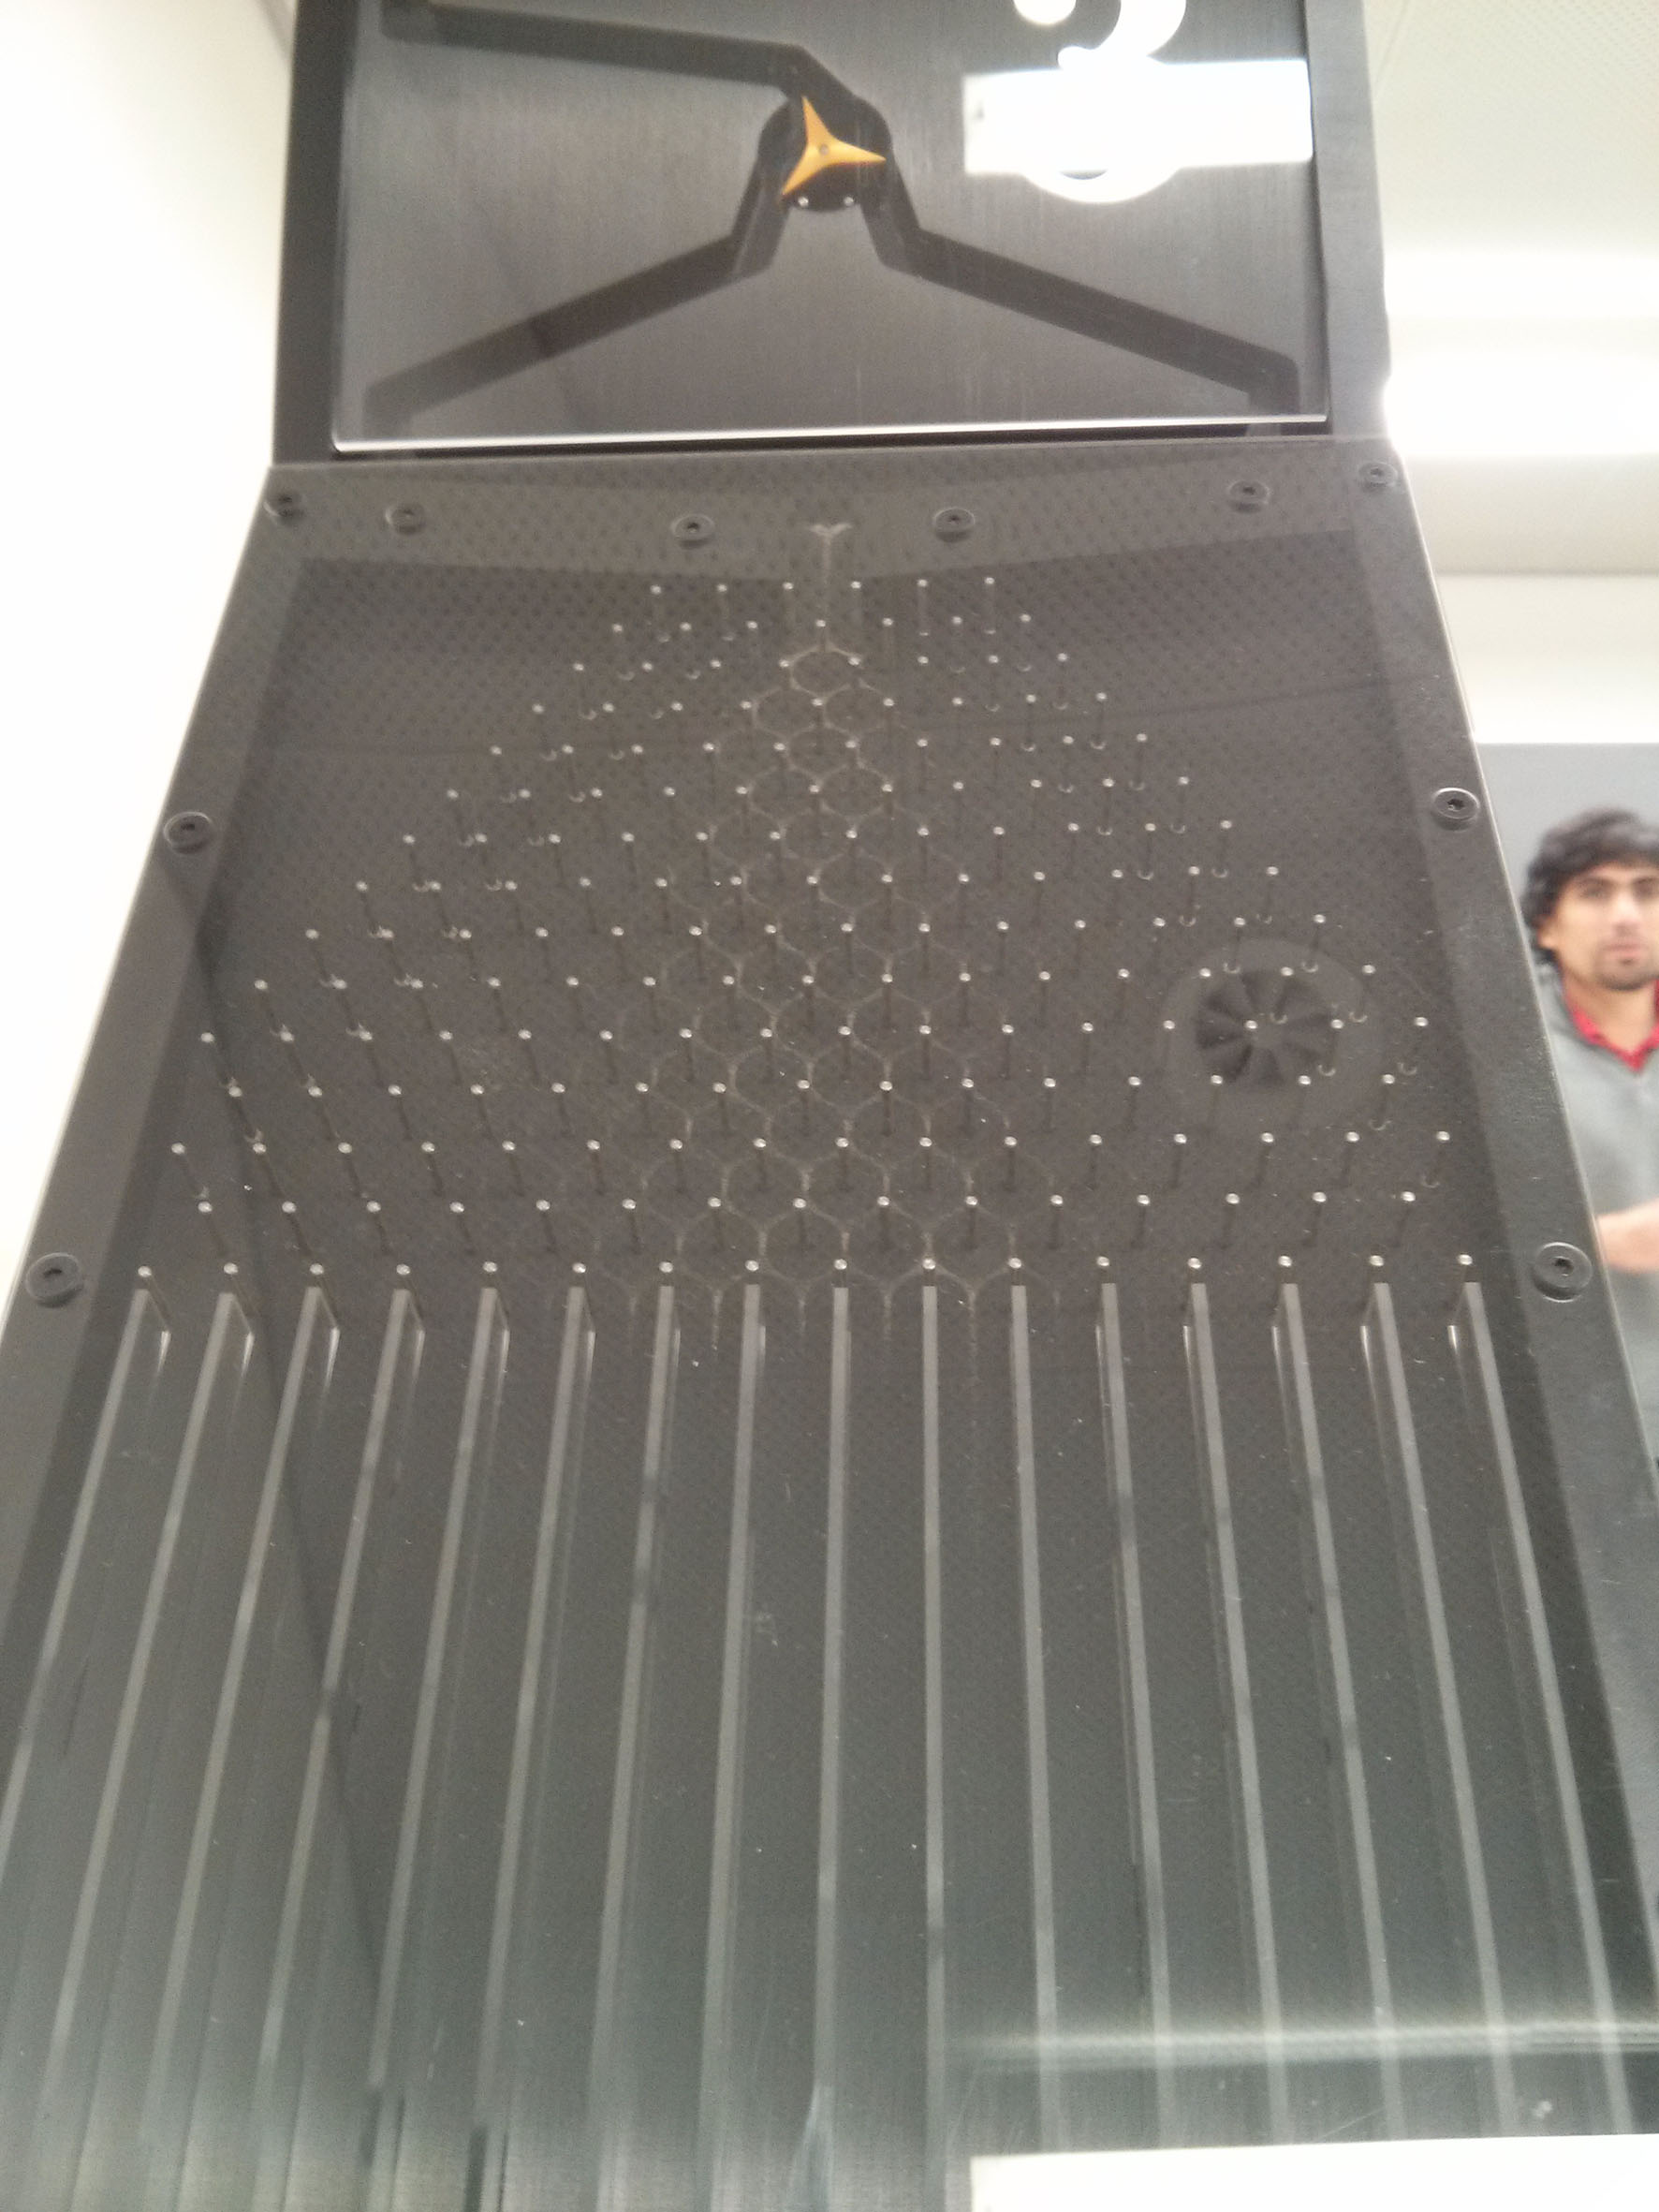
\includegraphics[width=0.7\textwidth]{img/Galton.png}
        \caption{The Galton box used in the experiment}
\end{figure}

For this experiment a series of 50 small metal balls is inserted 20 times into the box, one ball at a time to hinder interaction between the balls. After each series, the amount of balls in each slot is written down and after all series have been concluded, it is summed up to produce a distribution of 1000 balls.\\
During the whole course of the experiment we kept the board level using a water bubble leveler. We measured the tilt of the board to be $\ang{60}$ to the horizontal axis.

\section{Measurements}

% Table generated by Excel2LaTeX from sheet 'Tabelle2'
\begin{table}[H]
  \centering
    \begin{tabular}{|r||c|c|c|c|c|c|c|c|c|c|c|c|c|c|c|}
    \hline
          & Slot  &       &       &       &       &       &       &       &       &       &       &       &       &       & \\
    \hline
    Series & \textbf{0} & \textbf{1} & \textbf{2} & \textbf{3} & \textbf{4} & \textbf{5} & \textbf{6} & \textbf{7} & \textbf{8} & \textbf{9} & \textbf{10} & \textbf{11} & \textbf{12} & \textbf{13} & \textbf{14} \\ \hline\hline
    \textbf{1} & 0     & 0     & 1     & 0     & 3     & 10    & 10    & 11    & 6     & 4     & 5     & 0     & 0     & 0     & 0 \\
    \textbf{2} & 0     & 0     & 1     & 2     & 3     & 6     & 9     & 7     & 15    & 2     & 2     & 2     & 1     & 0     & 0 \\
    \textbf{3} & 0     & 0     & 0     & 2     & 1     & 6     & 13    & 7     & 12    & 4     & 2     & 1     & 2     & 0     & 0 \\
    \textbf{4} & 0     & 0     & 1     & 3     & 3     & 4     & 8     & 8     & 17    & 3     & 2     & 1     & 0     & 0     & 0 \\
    \textbf{5} & 0     & 0     & 1     & 2     & 5     & 3     & 11    & 12    & 6     & 7     & 2     & 1     & 0     & 0     & 0 \\
    \textbf{6} & 0     & 0     & 1     & 3     & 3     & 6     & 12    & 8     & 10    & 6     & 0     & 1     & 0     & 0     & 0 \\
    \textbf{7} & 0     & 0     & 0     & 1     & 2     & 5     & 8     & 8     & 9     & 11    & 3     & 3     & 0     & 0     & 0  \\
    \textbf{8} & 0     & 0     & 0     & 0     & 4     & 4     & 13    & 7     & 13    & 4     & 2     & 3     & 0     & 0     & 0 \\
    \textbf{9} & 0     & 1     & 1     & 2     & 5     & 2     & 6     & 16    & 8     & 5     & 3     & 0     & 1     & 0     & 0 \\
    \textbf{10} & 0     & 0     & 1     & 0     & 3     & 3     & 9     & 10    & 17    & 4     & 0     & 2     & 1     & 0     & 0  \\
    \textbf{11} & 0     & 0     & 0     & 1     & 5     & 2     & 12    & 10    & 13    & 4     & 2     & 0     & 1     & 0     & 0 \\
    \textbf{12} & 0     & 0     & 0     & 1     & 3     & 3     & 8     & 9     & 14    & 8     & 1     & 3     & 0     & 0     & 0\\
    \textbf{13} & 0     & 0     & 0     & 2     & 3     & 7     & 8     & 6     & 11    & 9     & 2     & 2     & 0     & 0     & 0 \\
    \textbf{14} & 0     & 0     & 0     & 1     & 4     & 6     & 7     & 13    & 9     & 6     & 1     & 2     & 1     & 0     & 0 \\
    \textbf{15} & 0     & 0     & 0     & 3     & 4     & 4     & 9     & 6     & 11    & 8     & 4     & 1     & 0     & 0     & 0\\
    \textbf{16} & 0     & 0     & 2     & 0     & 6     & 6     & 7     & 12    & 7     & 4     & 5     & 1     & 0     & 0     & 0 \\
    \textbf{17} & 0     & 0     & 2     & 0     & 8     & 5     & 10    & 9     & 5     & 7     & 4     & 0     & 0     & 0     & 0 \\
    \textbf{18} & 0     & 0     & 1     & 6     & 4     & 10    & 11    & 7     & 3     & 5     & 2     & 1     & 0     & 0     & 0  \\
    \textbf{19} & 0     & 1     & 0     & 1     & 3     & 9     & 10    & 5     & 12    & 5     & 1     & 3     & 0     & 0     & 0 \\
    \textbf{20} & 0     & 0     & 0     & 0     & 6     & 6     & 9     & 13    & 8     & 4     & 3     & 1     & 0     & 0     & 0  \\
    \hline\hline
    \textbf{Total} & 0     & 2     & 12    & 30    & 78    & 107   & 190   & 184   & 206   & 110   & 46    & 28    & 7     & 0     & 0 \\
    \hline
    \end{tabular}%
  \caption{Number of balls in each slot for all 20 series}
\end{table}%

So after the first runthrough, we have observed the following ball distribution:

\begin{figure}[H]
    \center   
        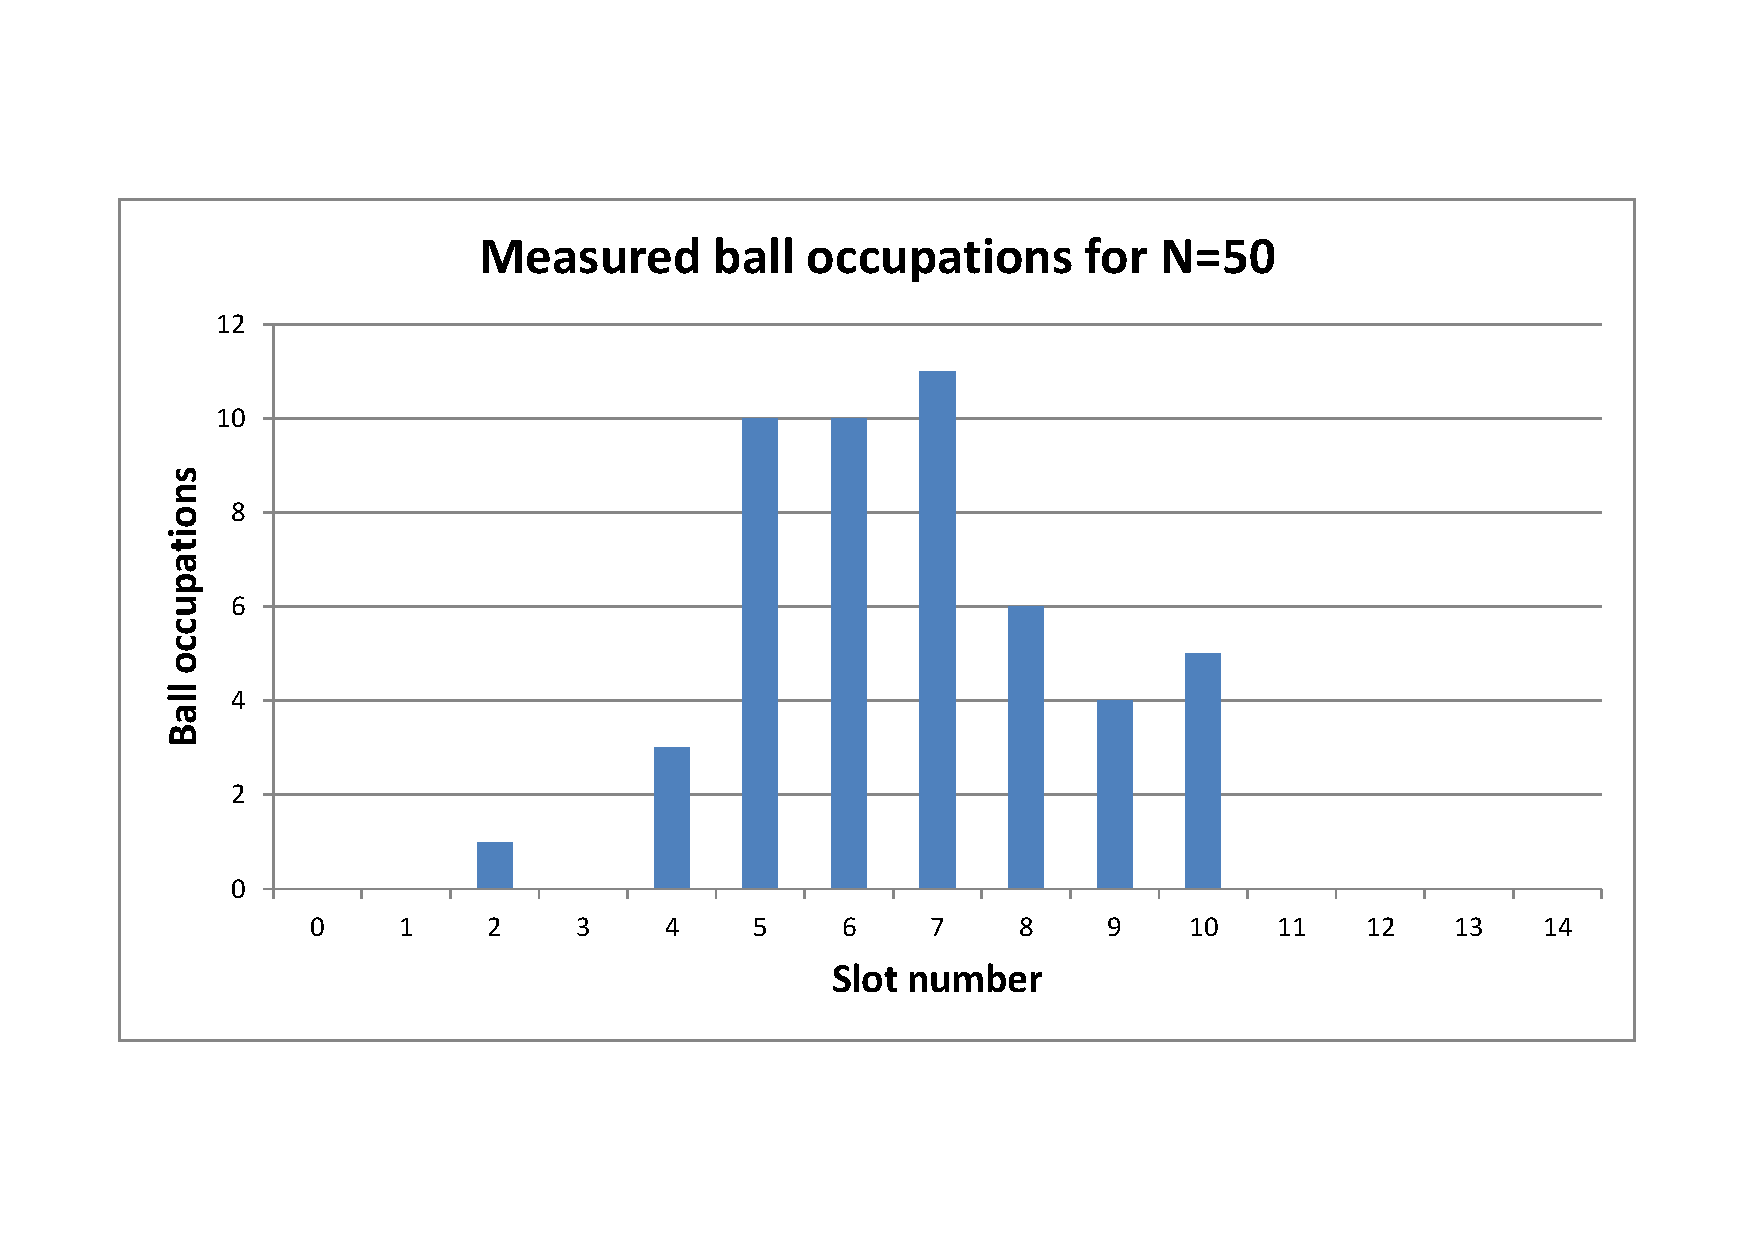
\includegraphics[width=0.9\textwidth]{img/ball_occup_n_50}
        \caption{The measured distribution after $N=50$ balls}
\end{figure}

which yields for mean $\bar{x}$, standard deviation $s_x,$ and standard error of mean $s_{\bar{x}}$
\begin{align*}
\bar{x} \pm s_{\bar{x}} &= 6.700 \pm 0.259\\
s_x &= 1.832
\end{align*}

For the accumulated measurement ($N=1000)$, we have observed the following distribution

\begin{figure}[H]
    \center   
        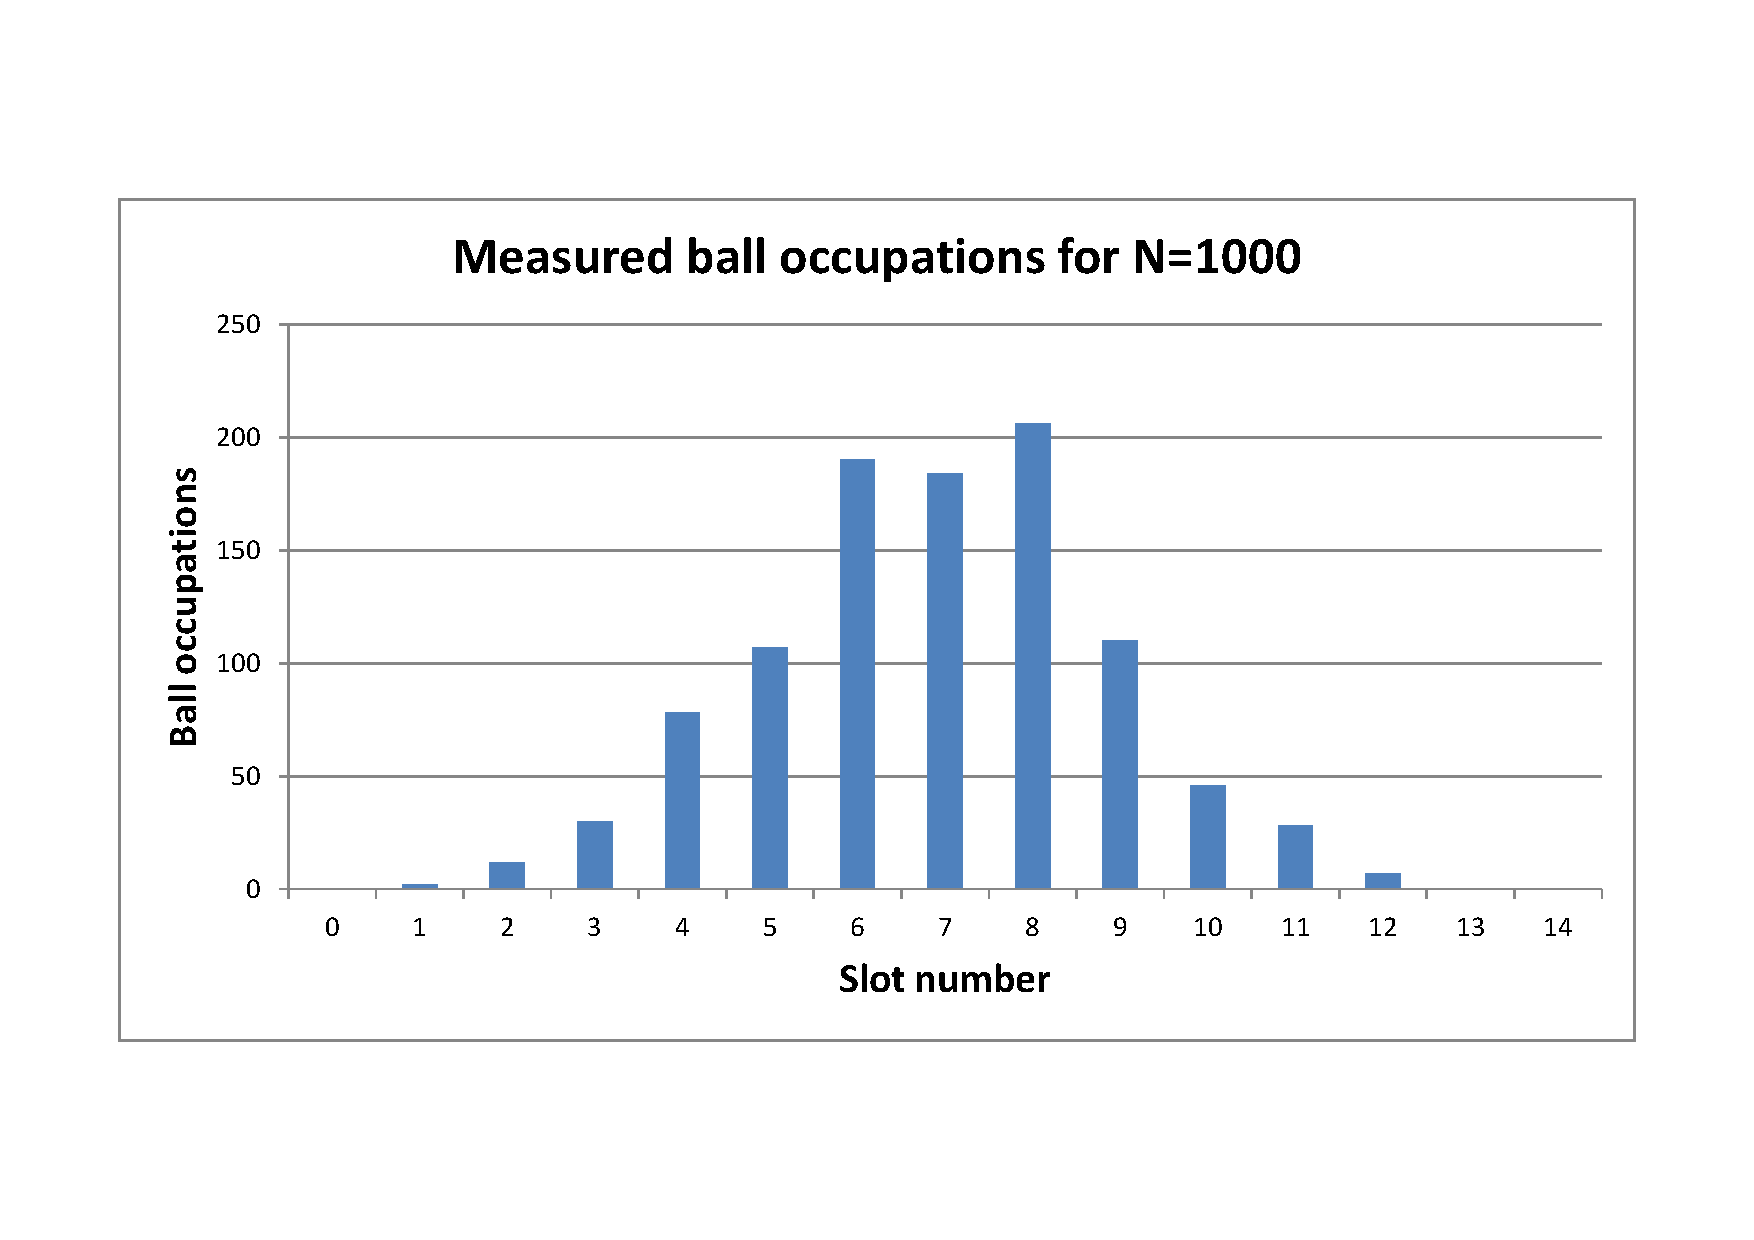
\includegraphics[width=0.9\textwidth]{img/ball_occup_n_1000}
        \caption{The measured distribution after $N=1000$ balls}
\end{figure}

which yields for mean $\bar{x}$, standard deviation $s_x,$ and standard error of mean $s_{\bar{x}}$
\begin{align*}
\bar{x} \pm s_{\bar{x}} &= 6.881 \pm 0.062\\
s_x &= 1.961
\end{align*}

\paragraph*{Comparison to Model}

\begin{center}
    \begin{tabular}{|c|ccc|ccc|}
    \hline
    & \multicolumn{3}{c|}{$N=50$} & \multicolumn{3}{c|}{$N=1000$}\\ \hline
    & $\bar{x}$ & $s_{\bar{x}}$ & $s_x$ & $\bar{x}$ & $s_{\bar{x}}$ & $s_x$ \\
    \hline \hline
    Model & 7.000 & 0.265 & 1.871 & 7.000 & 0.059 & 1.871\\
    \hline
    Measurement & 6.800 & 0.259 & 1.832 & 6.881 & 0.062 & 1.961\\
    \hline
    \end{tabular}
\end{center}

\paragraph*{Occupations}
We would like to answer the question which slots are statistically significantly over- and underoccupied. For that we use the formula from the script. A slot is statistically over- or underoccupied if

\begin{equation*}
\lvert f(x)-F(x) \rvert > 2...3 \sqrt{F(x)}
\end{equation*}

Applying this rule to our accumulated measurements ($N=1000$), we can conclude that only the values in Slot 2 and 4 are statistically significantly overoccupied.

\begin{figure}[H]
    \center   
        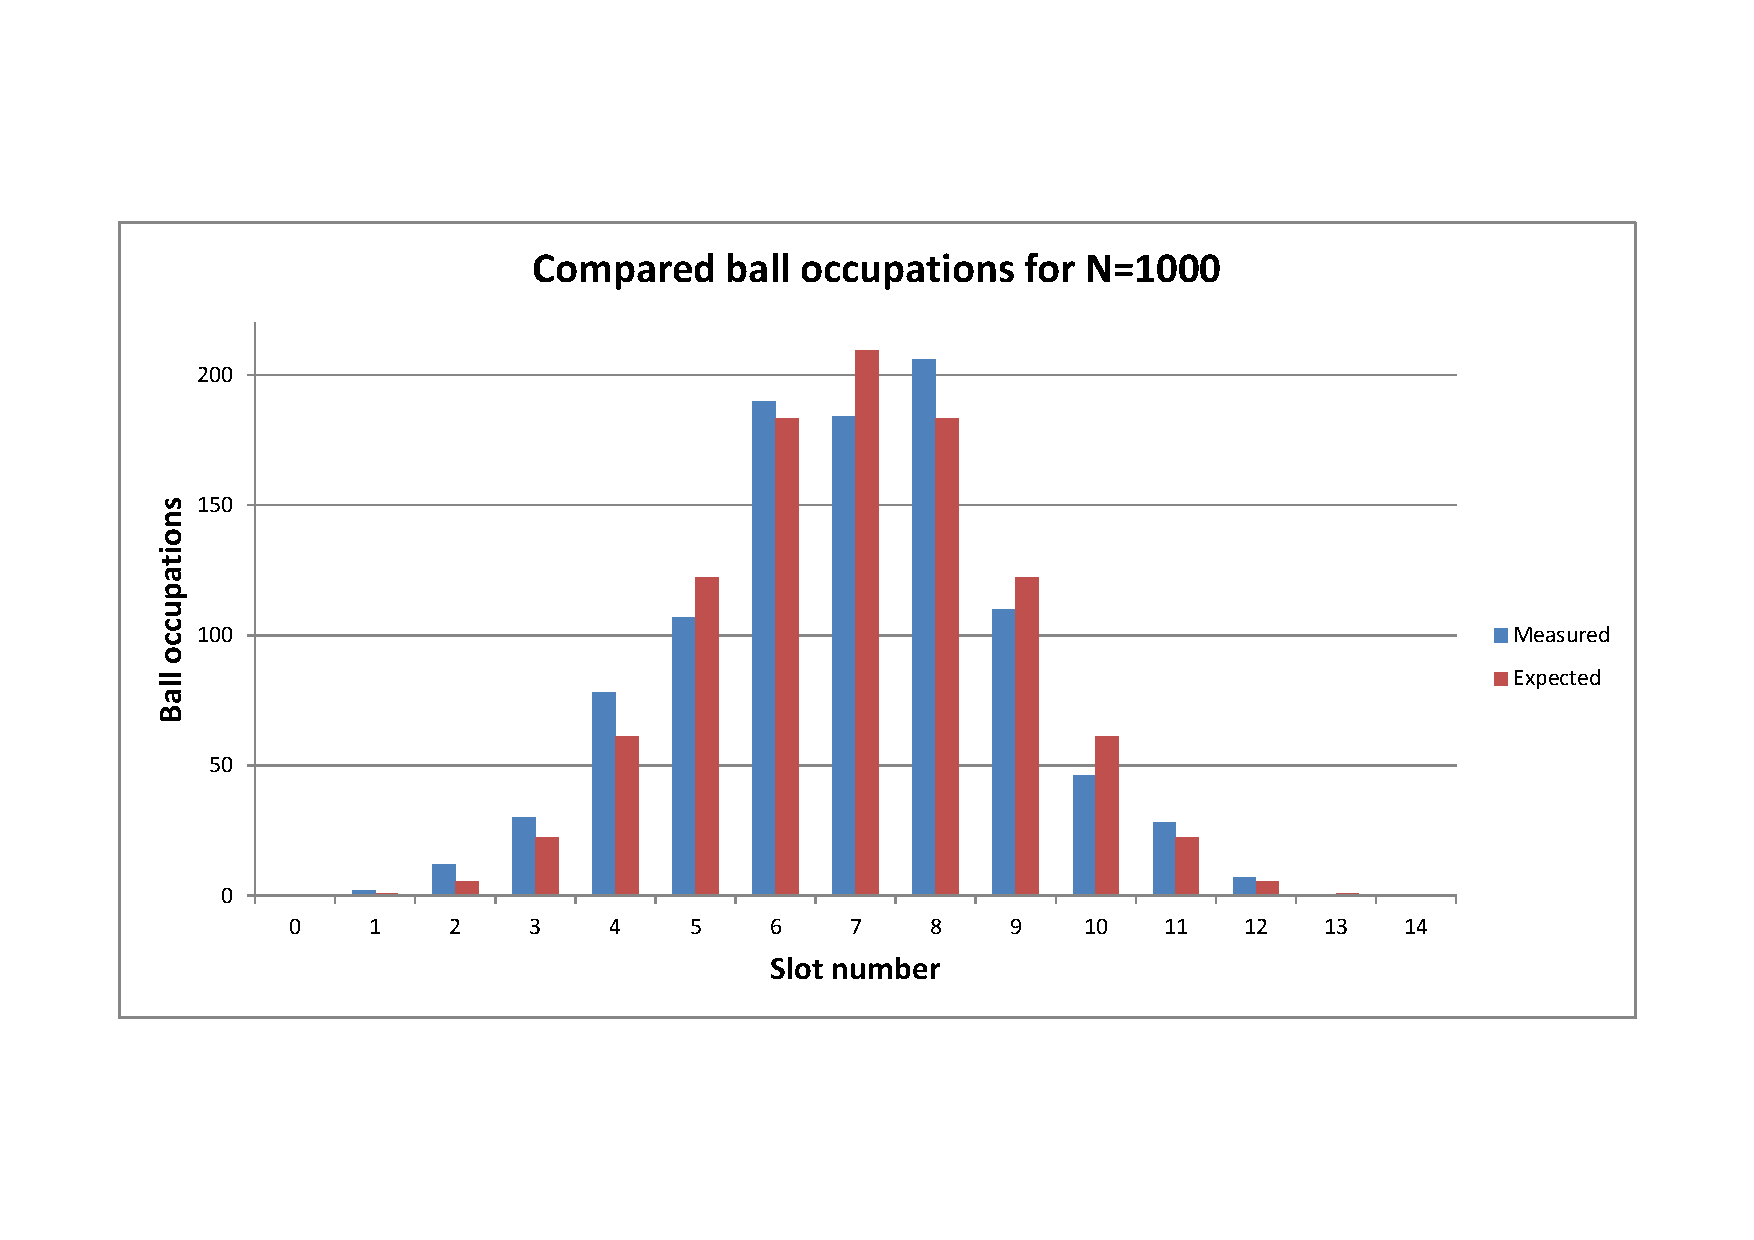
\includegraphics[width=1.0\textwidth]{img/ball_occup_1000_combo.pdf}
        \caption{Comparison of measured and expected slot occupations for $N=1000$ balls}
\end{figure}

\section{Discussion}
In our measurements, we noted some interesting anomalies. For starters, the slot in the center of the board has not been the most frequented in our runthrough, it was the one immediately right to it. Even the one left from the middle had a higher ball intake. Furthermore, the slots near to the right of the middle had more balls in them than the corresponding ones in the left. Far from the center, the situation is inverted and more balls are left than right. Apart from that, the distribution appears to be close to our expectations, even though the average slot is slightly too far on the left.

There are virtually no ways we could have influenced the experiment in order to get this result. We even tried to keep a steady distance between the balls by inserting them one at a time and keeping an eye on them while they fell down into the slots. We dismiss any concerns about the box not being ideally aligned horizontally, because for one we carefully adjusted it using a bubble level and also, there is no indication in the measured values for a clear tendency to the left or right. As is, we have to look at the box for an explanation. Probably the board has some minor build defects (e.g. bent pins or dells and dents in the material) which cause the left-right distribution at the pins to be uneven.

%-------------------------------Dice--------------------------------------------%

\chapter[Dice]{Dice (15 min)}

\section{Introduction}

\subsection{Experiment Goal}
The goal of this experiment is to demonstrate elementary statistical terms by experimental means. In order to do that, a die is thrown 144 times in a row. Afterwards, some statistical methods are applied for exercise

\subsection{Theory}
The theory for the first part is really simple. Assuming our Dice are completely fair, each value has the exact probability of $\frac{1}{6}$ of appearing.
 
\subsubsection{Expectations}

\paragraph{Single Die}
For one die thrown 144 times, the expected distribution is really boring, being completely even. We expect the following distribution

\begin{center}
    \begin{tabular}{|c|cccccc|}
    \hline
    Eye count & 1 & 2 & 3 & 4 & 5 & 6\\
    \hline
    Occurences & 24 & 24 & 24 & 24 & 24 & 24\\
    \hline
    \end{tabular}
\end{center}
and an arithmetic mean of $\mu = 3.5$ with variance $\sigma^2 = 2.937$ for each die throw.
\linebreak
Things get more interesting for two or four dice.

\paragraph{Double Die}
The expected occurences of the various eye counts for two ideal dice are:

\begin{center}
    \begin{tabular}{|c|ccccccccccc|}
    \hline
    Eye count & 2 & 3 & 4 & 5 & 6 & 7 & 8 & 9 & 10 & 11 & 12\\
    \hline
    Occurences & 2 & 4 & 6 & 8 & 10 & 12 & 10 & 8 & 6 & 4 & 2\\
    \hline
    \end{tabular}
\end{center}

with an arithmetic mean of $\mu = 7$ with variance $\sigma^2 = 5.915$ for each dice throw.

\paragraph{Quadruple Die}
For the following calculations, every 4 consecutive throws are conculded into one measurement. The classes for the thusly obtained measurements are quite clear, as the results are presented in descrete steps. We choose 21 classes, from 4 to 24.
The probability of such a class is described by the following formula\cite{dicewiki}, where $s$ is the number of sides of a die and $n$ the number of dice.

\begin{equation}
F_{s,n}(k)= \frac{1}{s^n}\cdot\sum_{i=0}^{\lfloor\frac{k-n}{s} \rfloor}(-i)^i\binom{n}{k}\cdot\binom{l-si-1}{n-1}
\end{equation}

Which yields an expected average value of $\mu=14$ and a variance of $\sigma^2=11.667$

\section[The Experiment]{Experiment Assembly and Execution}
Instead of being hardworking, we were clever, and used a box to speed up the whole experiment. We took the box and threw the dice in, six at a time. Once they were at rest, we carefully tilted the box in order to align them at an edge. This gave us the possibility to read six dice at a time without perturbing the order of the throws. In order to obtain 144 throws, we repeated the procedure 24 times.
\section{Measurements}

\begin{table}[H]
  \centering
    \begin{tabular}{|r||cccccccccccc|}
    \hline
    No.   & 1     & 2     & 3     & 4     & 5     & 6     & 7     & 8     & 9     & 10    & 11    & 12 \\
    rolled & 3     & 2     & 2     & 2     & 4     & 3     & 4     & 2     & 4     & 2     & 5     & 5 \\ \hline\hline
    No.   & 13    & 14    & 15    & 16    & 17    & 18    & 19    & 20    & 21    & 22    & 23    & 24 \\
    rolled & 2     & 4     & 4     & 1     & 3     & 4     & 1     & 1     & 5     & 6     & 6     & 6 \\ \hline\hline
    No.   & 25    & 26    & 27    & 28    & 29    & 30    & 31    & 32    & 33    & 34    & 35    & 36 \\
    rolled & 1     & 2     & 4     & 5     & 4     & 4     & 4     & 4     & 1     & 6     & 1     & 5 \\ \hline\hline
    No.   & 37    & 38    & 39    & 40    & 41    & 42    & 43    & 44    & 45    & 46    & 47    & 48 \\
    rolled & 6     & 2     & 4     & 6     & 6     & 3     & 6     & 5     & 2     & 6     & 2     & 6 \\ \hline\hline
    No.   & 49    & 50    & 51    & 52    & 53    & 54    & 55    & 56    & 57    & 58    & 59    & 60 \\
    rolled & 5     & 3     & 3     & 3     & 5     & 1     & 2     & 4     & 3     & 5     & 6     & 1 \\ \hline\hline
    No.   & 61    & 62    & 63    & 64    & 65    & 66    & 67    & 68    & 69    & 70    & 71    & 72 \\
    rolled & 1     & 5     & 1     & 2     & 5     & 6     & 5     & 6     & 1     & 1     & 3     & 2 \\ \hline\hline
    No.   & 73    & 74    & 75    & 76    & 77    & 78    & 79    & 80    & 81    & 82    & 83    & 84 \\
    rolled & 4     & 2     & 3     & 5     & 5     & 5     & 2     & 2     & 4     & 4     & 2     & 5 \\ \hline\hline
    No.   & 85    & 86    & 87    & 88    & 89    & 90    & 91    & 92    & 93    & 94    & 95    & 96 \\
    rolled & 1     & 1     & 3     & 6     & 3     & 2     & 5     & 3     & 3     & 6     & 5     & 5 \\ \hline\hline
    No.   & 97    & 98    & 99    & 100   & 101   & 102   & 103   & 104   & 105   & 106   & 107   & 108 \\
    rolled & 3     & 3     & 1     & 1     & 1     & 2     & 6     & 4     & 6     & 2     & 2     & 3 \\ \hline\hline
    No.   & 109   & 110   & 111   & 112   & 113   & 114   & 115   & 116   & 117   & 118   & 119   & 120 \\
    rolled & 5     & 3     & 2     & 5     & 4     & 6     & 2     & 2     & 3     & 1     & 4     & 1 \\ \hline\hline
    No.   & 121   & 122   & 123   & 124   & 125   & 126   & 127   & 128   & 129   & 130   & 131   & 132 \\
    rolled & 1     & 5     & 4     & 2     & 2     & 2     & 2     & 6     & 6     & 5     & 2     & 3 \\ \hline\hline
    No.   & 133   & 134   & 135   & 136   & 137   & 138   & 139   & 140   & 141   & 142   & 143   & 144 \\
    rolled & 2     & 4     & 4     & 5     & 2     & 6     & 5     & 5     & 2     & 1     & 6     & 6 \\ \hline
    \end{tabular}
    \caption{Measured rolled numbers for $N=144$ die throws}
\end{table}%

\subsection{Single Die}
We measured the following aggregate distribution for $N=144$ consequtive throws

\begin{center}
    \begin{tabular}{|c|cccccc|}
    \hline
    Eye count & 1 & 2 & 3 & 4 & 5 & 6\\
    \hline
    Occurences & 21 & 32 & 20 & 22 & 26 & 23\\
    \hline
    \end{tabular}
\end{center}
which yields an empirical arithmetic mean for the eye count of $\bar{x} = 3.479$ with variance $\sigma^2 = 2.909$

\subsection{Double Die}
We measured the following aggregate distribution for $N=72$ consequtive double die throws
\begin{center}
    \begin{tabular}{|c|ccccccccccc|}
    \hline
    Eye count & 2 & 3 & 4 & 5 & 6 & 7 & 8 & 9 & 10 & 11 & 12\\
    \hline
    Occurences & 4 & 4 & 5 & 7 & 13 & 6 & 14 & 5 & 7 & 5 & 2\\
    \hline
    \end{tabular}
\end{center}
which yields an empirical arithmetic mean for the eye count sum of $\bar{x} = 6.958$ with variance $\sigma^2 = 6.717$

\begin{figure}[H]
    \center   
        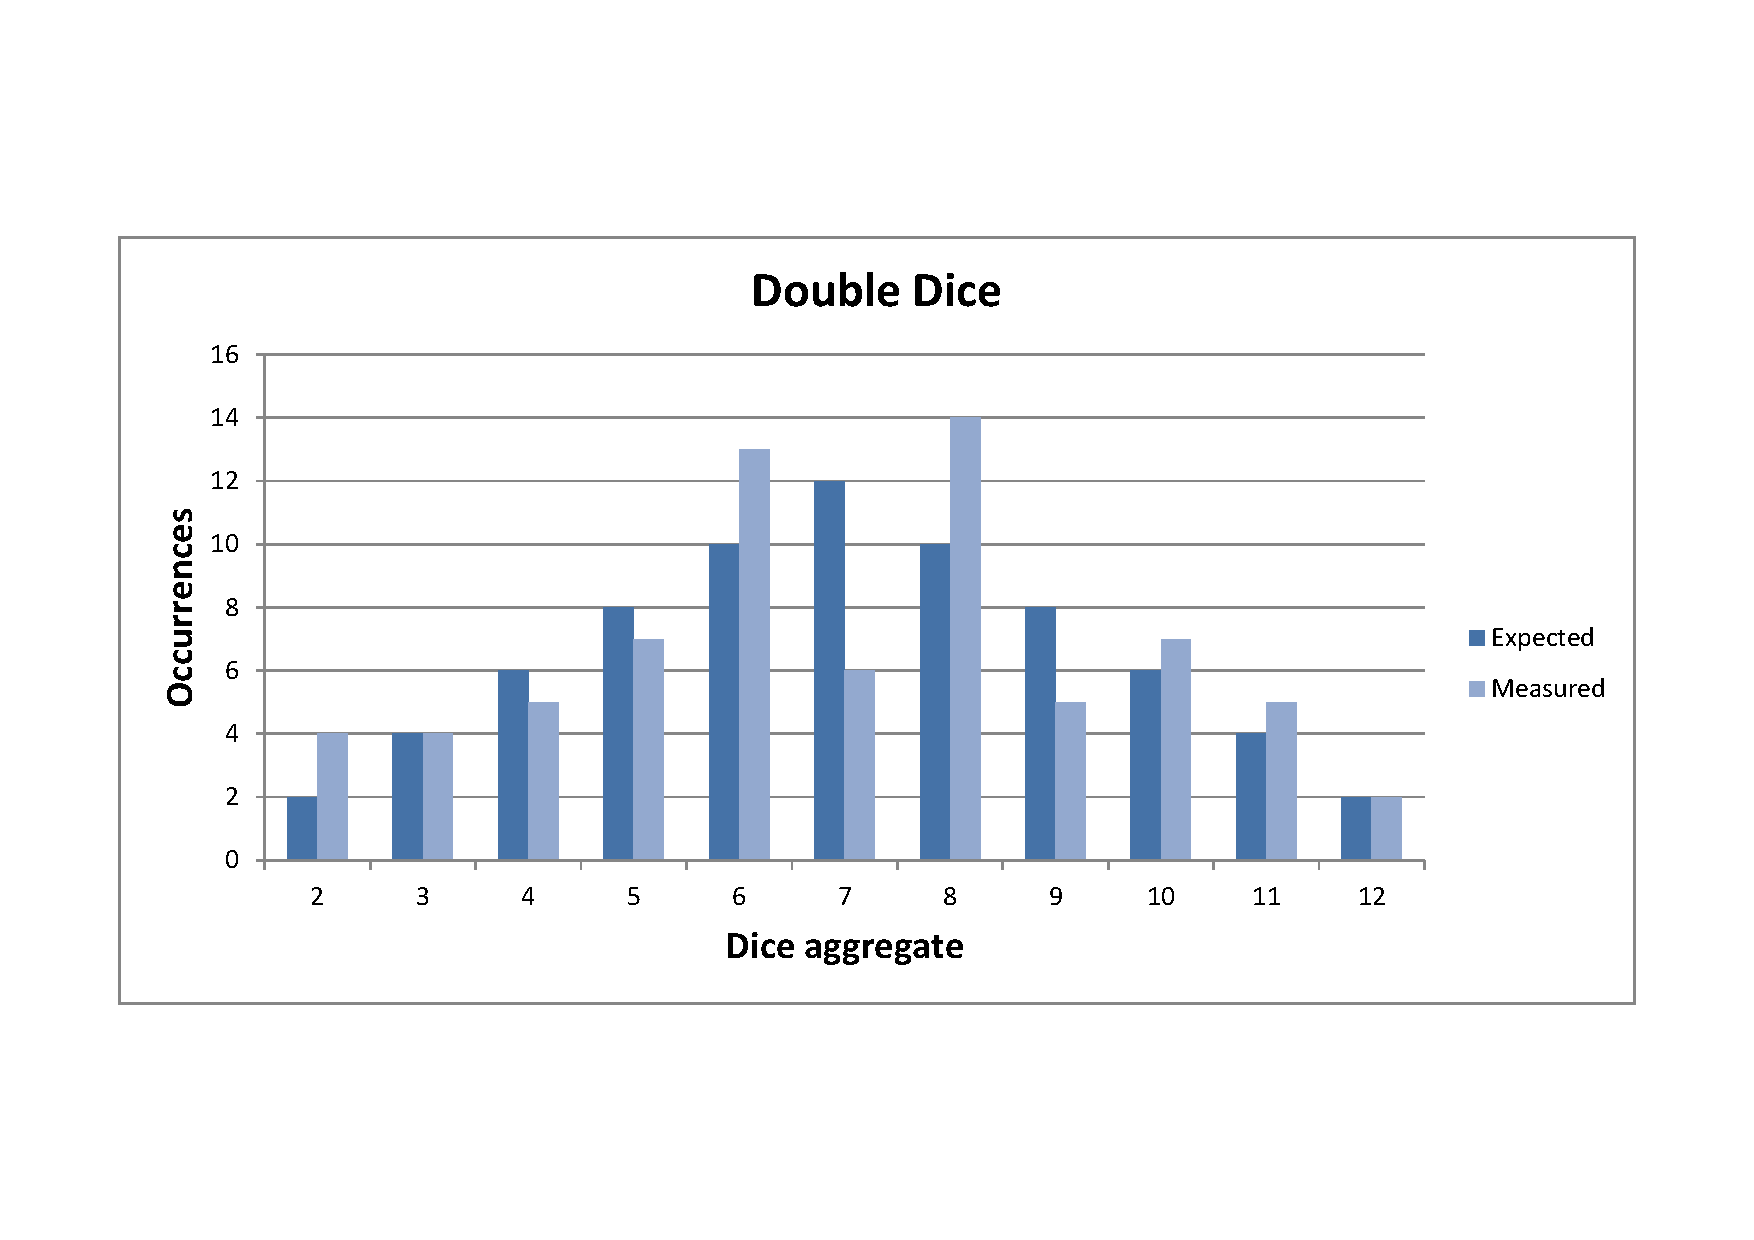
\includegraphics[width=1\textwidth]{img/double_dice_combo.pdf}
        \caption{Expected and measured values for $N=72$ consequtive double die throws}
\end{figure}

\subsection{Quadruple Die}
Accumulating our measurements for four dice each we get the following distribution:

\begin{center}
    \begin{tabular}{|c|ccccccccccc|}
    \hline
    Eye count & 4 & 5 & 6 & 7 & 8 & 9 & 10 & 11 & 12 & 13 & 14\\ 
    \hline
    Occurences & 0 & 0 & 0 & 1 & 1 & 4 & 0 & 2 & 4 & 5 & 4\\
    \hline\hline
    Eye count & 15 & 16 & 17 & 18 & 19 & 20 & 21 & 22 & 23 & 24 &\\
    \hline
    Occurences & 5 & 4 & 0 & 2 & 1 & 1 & 0 & 1 & 1 & 0 &\\
    \hline
    \end{tabular}
\end{center}

which yields an arithmetic mean for the eye count sum of $\bar{x} = 13.917$ with variance $\sigma^2 = 13.793$ for each throw\\

\section{Discussion}
It appears that our dice throwing skills are questionable at best. As there are no obvious error sources, we can assume this to be within the statistical frame of normality.

%-------------------------------Grav Constant-----------------------------------%
\chapter[Gravitational Acceleration]{Determining the local Gravitational Acceleration (80 min)}
\section{Introduction}
By dropping an object from a known height and measuring the time it takes to hit the floor we can calculate the local gravitational acceleration. Determining said local gravitational acceleration will be the topic of this experiment.

\subsection{Experiment Goal}
First and foremost this experiment is intended to get well acquainted with uncertainty estimation and error calculation. Determining the exact value of the gravitational acceleration is only relevant to a certain degree since we are only provided with a set of standard household equipment and tools with limited accuracy.

\subsection{Theory}
The falltime of an object dropped from a height $h$ is, negtlecting air resistance, given by rearranging the generally known formula 
\begin{equation}h = \frac{1}{2} g t_{\text{fall}}^{2} \Longleftrightarrow  t_{\text{fall}} = \sqrt{\frac{2h}{g}}
\end{equation}
With that formula in mind we would expect the following falltimes for heights $h_1 = 1\unit{m}$ and $h_2 = 1.2\unit{m}$ with $g = 9.81\unit{\frac{m}{s^{2}}}$

\begin{center}
    \begin{tabular}{|l||l|}
    \hline
    Height [m] & Falltime [s]\\ \hline \hline
    1 & 0.452\\ \hline
    1.2 & 0.495\\ \hline
    \end{tabular}
\end{center}

We can use the formula stated in the script \cite[p. 54, f. 4.2]{physcript13} to approximate the value of $g$ in dependance of geographic latitude $\Phi$ and height above sea level $H$
\begin{equation} 
g = 9.80616 - 0.025928 \cdot \cos(2\Phi) + 0 .000069 \cdot \cos^{2} \Phi - 3.086 \cdot 10^{-7} H
\end{equation}
which yields a value of $g = 9.80783\unit{ms^{-2}}$ for Bern ($H = 550\unit{m}, \Phi = \ang{47}$). This value is very close to the value $g = 9.80919\unit{\frac{m}{s^{2}}}$ calculated by WolframAlpha based on the EGM2008 12th order model.\\

\paragraph*{Finding $\mathbf{g}$}
Given a fall time $t_{\text{fall}}$ of an object dropped from a height $h$, it is very easy to calculate $g$ in terms of $t_{\text{fall}}$ and $h$:

\begin{equation} \label{eq:find}
g=\frac{2h}{t_{\text{fall}}^2}
\end{equation}

\section{Experiment assembly and execution}
We set the height of the provided unipod to $h=1.2\unit{m}\pm 0.003\unit{m}$. Instead of the provided shims we used the balls from the Galton Box experiment. The balls should exhibit better flight characteristics due to their bigger mass and more aerodynamic shape. The balls were held up high by an electro-magnet which could be switched of instantly by an attached trigger button. The power supply providing power to the electro-magnet on top of the unipod was set to 12$\unit{V}$ for maximum attraction force. To achieve the most accurate measurements possible we first had a couple of trial runthroughs in order to get a better feeling for the ball's fall charasteristics. An ordinary no-name stop watch was used to measure the fall time (accurate to 1/100th of a second). Each of us measured the fall times of 100 balls, totalling up to 200 fall time measurements.

\section{Measurements}
We measured the following fall times $t_{\text{fall}}$ during the course of the experiment:

\begin{table}[H]
  \centering
    \begin{tabular}{|r||cccccccccccc|}
     \hline
    No.   & 1     & 2     & 3     & 4     & 5     & 6     & 7     & 8     & 9     & 10    & 11    & 12 \\ 
    $t_{\text{falll}}$[hs] & 50    & 44    & 50    & 41    & 43    & 48    & 48    & 45    & 45    & 48    & 45    & 42 \\ \hline \hline
    No.   & 13    & 14    & 15    & 16    & 17    & 18    & 19    & 20    & 21    & 22    & 23    & 24 \\ 
    $t_{\text{falll}}$[hs] & 45    & 42    & 42    & 43    & 45    & 45    & 43    & 42    & 46    & 46    & 45    & 42 \\ \hline \hline
    No.   & 25    & 26    & 27    & 28    & 29    & 30    & 31    & 32    & 33    & 34    & 35    & 36 \\
    $t_{\text{falll}}$[hs] & 45    & 45    & 45    & 43    & 43    & 42    & 46    & 46    & 45    & 42    & 45    & 43 \\ \hline \hline
    No.   & 37    & 38    & 39    & 40    & 41    & 42    & 43    & 44    & 45    & 46    & 47    & 48 \\ 
    $t_{\text{falll}}$[hs] & 45    & 45    & 42    & 43    & 43    & 46    & 45    & 43    & 40    & 40    & 43    & 43 \\ \hline \hline
    No.   & 49    & 50    & 51    & 52    & 53    & 54    & 55    & 56    & 57    & 58    & 59    & 60 \\ 
    $t_{\text{falll}}$[hs] & 43    & 43    & 48    & 43    & 45    & 46    & 43    & 45    & 45    & 42    & 42    & 42 \\ \hline \hline
    No.   & 61    & 62    & 63    & 64    & 65    & 66    & 67    & 68    & 69    & 70    & 71    & 72 \\ 
    $t_{\text{falll}}$[hs] & 46    & 48    & 45    & 48    & 46    & 45    & 45    & 45    & 42    & 45    & 42    & 43 \\ \hline \hline
    No.   & 73    & 74    & 75    & 76    & 77    & 78    & 79    & 80    & 81    & 82    & 83    & 84 \\
    $t_{\text{falll}}$[hs] & 46    & 45    & 43    & 42    & 43    & 45    & 43    & 43    & 42    & 42    & 45    & 46 \\ \hline \hline
    No.   & 85    & 86    & 87    & 88    & 89    & 90    & 91    & 92    & 93    & 94    & 95    & 96 \\ 
    $t_{\text{falll}}$[hs] & 43    & 42    & 45    & 48    & 42    & 46    & 42    & 46    & 45    & 45    & 48    & 46 \\ \hline \hline
    No.   & 97    & 98    & 99    & 100   & 101   & 102   & 103   & 104   & 105   & 106   & 107   & 108 \\ 
    $t_{\text{falll}}$[hs] & 43    & 46    & 45    & 46    & 45    & 45    & 45    & 45    & 42    & 43    & 42    & 46 \\ \hline \hline
    No.   & 109   & 110   & 111   & 112   & 113   & 114   & 115   & 116   & 117   & 118   & 119   & 120 \\ 
    $t_{\text{falll}}$[hs] & 43    & 45    & 45    & 46    & 43    & 43    & 42    & 46    & 42    & 43    & 45    & 40 \\ \hline \hline
    No.   & 121   & 122   & 123   & 124   & 125   & 126   & 127   & 128   & 129   & 130   & 131   & 132 \\ 
    $t_{\text{falll}}$[hs] & 45    & 46    & 43    & 45    & 45    & 45    & 46    & 43    & 46    & 43    & 45    & 48 \\ \hline \hline
    No.   & 133   & 134   & 135   & 136   & 137   & 138   & 139   & 140   & 141   & 142   & 143   & 144 \\
    $t_{\text{falll}}$[hs] & 42    & 46    & 46    & 45    & 46    & 50    & 45    & 48    & 42    & 45    & 48    & 51 \\ \hline \hline
    No.   & 145   & 146   & 147   & 148   & 149   & 150   & 151   & 152   & 153   & 154   & 155   & 156 \\ 
    $t_{\text{falll}}$[hs] & 46    & 46    & 45    & 46    & 51    & 43    & 45    & 46    & 45    & 48    & 46    & 45 \\ \hline \hline
    No.   & 157   & 158   & 159   & 160   & 161   & 162   & 163   & 164   & 165   & 166   & 167   & 168 \\ 
    $t_{\text{falll}}$[hs] & 45    & 43    & 45    & 46    & 43    & 46    & 46    & 46    & 43    & 45    & 46    & 48 \\ \hline \hline
    No.   & 169   & 170   & 171   & 172   & 173   & 174   & 175   & 176   & 177   & 178   & 179   & 180 \\ 
    $t_{\text{falll}}$[hs] & 42    & 45    & 45    & 45    & 48    & 45    & 45    & 40    & 43    & 46    & 43    & 48 \\ \hline \hline
    No.   & 181   & 182   & 183   & 184   & 185   & 186   & 187   & 188   & 189   & 190   & 191   & 192 \\ 
    $t_{\text{falll}}$[hs] & 43    & 42    & 43    & 42    & 46    & 42    & 50    & 42    & 43    & 45    & 48    & 45 \\ \hline \hline
    No.   & 193   & 194   & 195   & 196   & 197   & 198   & 199   & 200   &       &       &       &  \\ 
    $t_{\text{falll}}$[hs] & 43    & 45    & 46    & 43    & 45    & 48    & 43    & 45    &       &       &       &  \\ \hline
    \end{tabular}%
    \caption{Measured fall times $t_{\text{fall}}$ in $[\frac{1}{100}\unit{s}]=[\unit{hs}]$ for $N=200$ runthroughs}
\end{table}%

Applying standard statistical analysis yields the following statistical properties of our measurement series

\begin{center}
    \begin{tabular}{l l l}
	mean fall time & $\overline{t_{\text{fall}}}$ & 44.605 $\frac{1}{100}$s\\
	std. error of mean & $s_{\overline{t_{\text{fall}}}}$ & 0.149 $\frac{1}{100}$s\\
	std. deviation of $t_{\text{fall}}$ & $s_{t_{\text{fall}}}$ & 2.110 $\frac{1}{100}$s\\
	height & $h$ & 1.200m\\
	height meas. inaccuracy & $s_h$ & 0.003m   
    \end{tabular}
\end{center}

Using equation \ref{eq:find} and 

\begin{equation}
\bar{g} = \frac{2 \bar{h}}{\overline{t_{\text{fall}}}^2}
\end{equation}

as well as 

\begin{equation}
s_{\bar{g}}^2 = \bar{h}^2 \cdot s_{\overline{t_{\text{fall}}}}^2 + \overline{t_{\text{fall}}}^2 \cdot s_{\bar{h}}^2
\end{equation}

we can now find the value of $g$:

\begin{equation}
g = \bar{g} \pm s_{\bar{g}} = 12.063\unit{m s^{-2}} \pm 0.223\unit{m s^{-2}}
\end{equation}

\section{Discussion}
We expected to measure a value of $g = 9.808\unit{ms^{-2}}$, but instead we found the value of $g$ to be $12.063\unit{m s^{-2}} \pm 0.223\unit{m s^{-2}}$ which is about $22.99\%$ higher.\\
Apparently our way of measuring the ball's fall time had some serious flaws.\\
Firstly, we set the height of the unipod too low, so the deviations from the ideal value have a much higher significance. We should have set the unipod as high as possible.\\
Secondly, measuring time with a handheld stopwatch is inherently inaccurate. We tried to synchronize the peeping sound of the watch to the ball's impact sound. After recognizing that our values for the fall times were too low, we analyzed the peeping behaviour of the stopwatch by looking at a video of the watch being started and stopped frame by frame. We measured the duration of the beep to be about $0.1$s. Assuming we did not synchronize the ball's impact sound to the beginning of the stop beep but about $0.03$s into the beep sound, the resulting value for $g$ would be a much better fit.

\begin{thebibliography}{9}

\bibitem{physcript13}
  Peter Wurz,
  \emph{Anleitung zum Physikpraktikum}
  FS2013
  
\bibitem{dicewiki}
	Dice on Wikipedia
	\emph{http://en.wikipedia.org/wiki/Dice\#Probability}
	11.03.2013

\end{thebibliography}

\end{document}
